% Compile: pdflatex run_context_architecture.tex
% Requires: tikz, geometry, xcolor
\documentclass[tikz,border=10pt]{standalone}
\usepackage{tikz}
\usetikzlibrary{
  arrows.meta,
  backgrounds,
  calc,
  fit,
  positioning,
  shadows.blur,
  shapes.geometric,
  shapes.multipart
}

\definecolor{globalFill}{HTML}{E8F4FC}
\definecolor{subFill}{HTML}{F0F7E8}
\definecolor{artFill}{HTML}{FFF4E6}
\definecolor{cfgFill}{HTML}{F3E8FF}
\definecolor{fsFill}{HTML}{F8F9FA}
\definecolor{accent}{HTML}{2B6CB0}
\definecolor{accentGreen}{HTML}{2F855A}
\definecolor{accentOrange}{HTML}{C05621}

% Text helpers inside node bodies (not TikZ keys)
\newcommand{\field}[1]{{\ttfamily\footnotesize\textcolor{black!75}{#1}}}
\newcommand{\method}[1]{{\ttfamily\footnotesize\textcolor{accent}{#1}}}

\tikzset{
  class/.style={
    draw=#1!70!black,
    fill=#1,
    rounded corners=3pt,
    line width=0.8pt,
    align=left,
    font=\small\sffamily,
    inner sep=6pt
  },
  arr/.style={-{Stealth[length=2.2mm]}, line width=0.9pt, draw=black!55},
  comp/.style={arr, draw=accent},
  derive/.style={arr, densely dashed, draw=accentGreen},
  handoff/.style={arr, line width=1.1pt, draw=accentOrange},
  note/.style={font=\footnotesize\sffamily, text=black!65, align=center},
  fsbox/.style={
    draw=black!25,
    fill=fsFill,
    rounded corners=2pt,
    font=\ttfamily\scriptsize,
    inner sep=4pt,
    align=left
  },
  worker/.style={
    draw=accentOrange!60!black,
    fill=accentOrange!12,
    rounded corners=2pt,
    font=\footnotesize\sffamily,
    inner sep=3pt
  }
}

\begin{document}
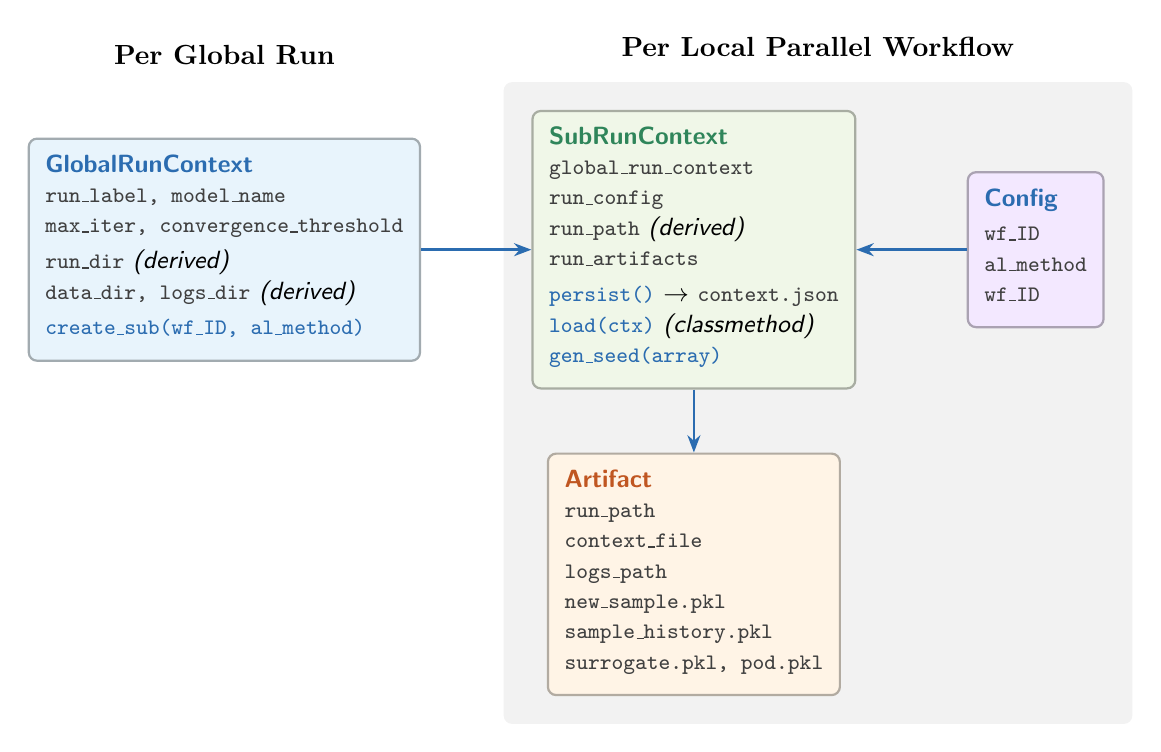
\begin{tikzpicture}[node distance=8mm and 14mm]

% --- Dataclass nodes ---
\node[class=globalFill] (global) {
  \textcolor{accent}{\textbf{GlobalRunContext}}\\[2pt]
  \begin{tabular}{@{}l@{}}
    \field{run\_label, model\_name}\\
    \field{max\_iter, convergence\_threshold}\\[2pt]
    \field{run\_dir} \textit{(derived)}\\
    \field{data\_dir, logs\_dir} \textit{(derived)}\\[2pt]
    \method{create\_sub(wf\_ID, al\_method)}
  \end{tabular}
};

\node[above=of global] {\textbf{Per Global Run}};

\node[class=subFill, right=of global] (sub) {
  \textcolor{accentGreen}{\textbf{SubRunContext}}\\[2pt]
  \begin{tabular}{@{}l@{}}
    \field{global\_run\_context}\\
    \field{run\_config}\\
    \field{run\_path} \textit{(derived)}\\
    \field{run\_artifacts}\\[2pt]
    \method{persist()} $\rightarrow$ \field{context.json}\\
    \method{load(ctx)} \textit{(classmethod)}\\
    \method{gen\_seed(array)}
  \end{tabular}
};

\node[class=cfgFill, right=of sub] (config) {
  \textcolor{accent}{\textbf{Config}}\\[2pt]
  \begin{tabular}{@{}l@{}}
    \field{wf\_ID}\\
    \field{al\_method}\\
    \field{wf\_ID}
  \end{tabular}
};

\node[class=artFill, below=of sub] (artifact) {
  \textcolor{accentOrange}{\textbf{Artifact}}\\[2pt]
  \begin{tabular}{@{}l@{}}
    \field{run\_path}\\
    \field{context\_file}\\
    \field{logs\_path}\\
    \field{new\_sample.pkl}\\
    \field{sample\_history.pkl}\\
    \field{surrogate.pkl, pod.pkl}
  \end{tabular}
};

\draw[comp] (config.west) -- (sub.east);
\draw[comp] (sub.south) -- (artifact.north);
\draw[comp] (global.east) -- (sub.west);

\begin{scope}[on background layer]
  \node[fill=black!5, rounded corners=3pt, inner sep=10pt,
        fit=(sub)(config)(artifact)](frame) {};
        
\end{scope}

\node[above=of frame, yshift=-6mm] {\textbf{Per Local Parallel Workflow}};

% % --- Composition ---
% \draw[comp] (global.south east) -- ++(0,-4mm) -| (sub.north);
% \draw[comp] (config.north) -- (config.north |- sub.west) coordinate (cjoin)
%       (cjoin) -- (sub.west);
% \node[note, left=2mm of config] {per workflow};
% \draw[comp] (sub.south) -- (artifact.north) node[midway, right=1mm, note] {owns};

% % --- Derivation from global ---
% \node[fsbox, right=18mm of global, minimum width=42mm] (gpath) {
%   \textbf{run\_dir} =\\[-1pt]
%   \texttt{cwd/training\_runs/}\\
%   \texttt{\{model\}/\{run\_label\}/}
% };
% \draw[derive] (global.east) -- (gpath.west);

% % --- Filesystem tree ---
% \node[fsbox, below=12mm of gpath, minimum width=52mm, anchor=north west] (fstree) at (gpath.south west) {
% \textbf{On-disk layout}\\[2pt]
% \texttt{training\_runs/model/run\_label/}\\
% \quad\texttt{data/} \hfill \textit{shared simulations}\\
% \quad\texttt{logs/} \hfill \textit{global logs}\\
% \quad\texttt{wf\_0/}\\
% \quad\quad\texttt{context.json}\\
% \quad\quad\texttt{new\_sample.pkl}\\
% \quad\quad\texttt{sample\_history.pkl}\\
% \quad\quad\texttt{surrogate.pkl, pod.pkl}\\
% \quad\quad\texttt{logs/}\\
% \quad\texttt{wf\_1/} \hfill \textit{$\cdots$}
% };

% \draw[derive] (sub.east) -- ++(8mm,0) |- (fstree.north)
%   node[pos=0.25, above, note] {mkdir + paths};

% % --- Workflow handoff ---
% \node[worker, above=14mm of global, xshift=-55mm] (driver) {Workflow driver\\\textit{e.g.\ \texttt{wf\_update.py}}};
% \node[worker, above=14mm of global, xshift=55mm] (workers) {Subprocess tasks\\\textit{sim, train, AL, MSE}};

% \draw[handoff] (driver.south) -- ++(0,-3mm) -| (global.north)
%   node[near start, above, note] {construct};
% \draw[handoff] (global.north) -- ++(0,5mm) -| (driver.south);

% \draw[handoff] (sub.east) -- ++(12mm,0) node[right, note, align=left] {writes\\[-2pt]\texttt{context.json}}
%   |- ($(workers.south)+(0,-3mm)$) -- (workers.south);
% \draw[handoff] (workers.south) -- ++(0,-3mm) -| (sub.north east)
%   node[pos=0.75, above, note] {\texttt{SubRunContext.load(-{}-ctx)}};

% % --- context.json payload ---
% \node[fsbox, left=18mm of sub, minimum width=44mm, yshift=-8mm] (json) {
%   \textbf{context.json snapshot}\\[2pt]
%   \texttt{schema\_version}\\
%   \texttt{global \{...\}}\\
%   \texttt{run\_config \{...\}}\\
%   \texttt{artifacts \{paths\}}
% };
% \draw[handoff] (sub.west) -- (json.east) node[midway, above, note] {persist / load};

% % --- Legend ---
% \begin{scope}[on background layer]
%   \node[draw=black!20, fill=white, rounded corners=3pt, inner sep=6pt,
%         fit=(driver)(workers)(fstree)(json)(global)(sub)(artifact)(config),
%         label={[font=\small\sffamily\bfseries]above:ROSE \texttt{workflows/run\_context.py}}] (frame) {};
% \end{scope}

% \node[below=3mm of frame.south, font=\footnotesize\sffamily, text=black!55] {
%   Solid: composition \quad
%   Dashed: derived paths \quad
%   Orange: \texttt{context.json} handoff between driver and tasks
% };

\end{tikzpicture}
\end{document}
